\paragraph{Example 1: No input arguments}
\begin{lstlisting}[language=Python]
from BNumMet.Visualizers.RandomVisualizer import RandomVisualizer
randomVisualizer = RandomVisualizer()
randomVisualizer.run()
\end{lstlisting}

\begin{enumerate}
    \item Initial State\\
    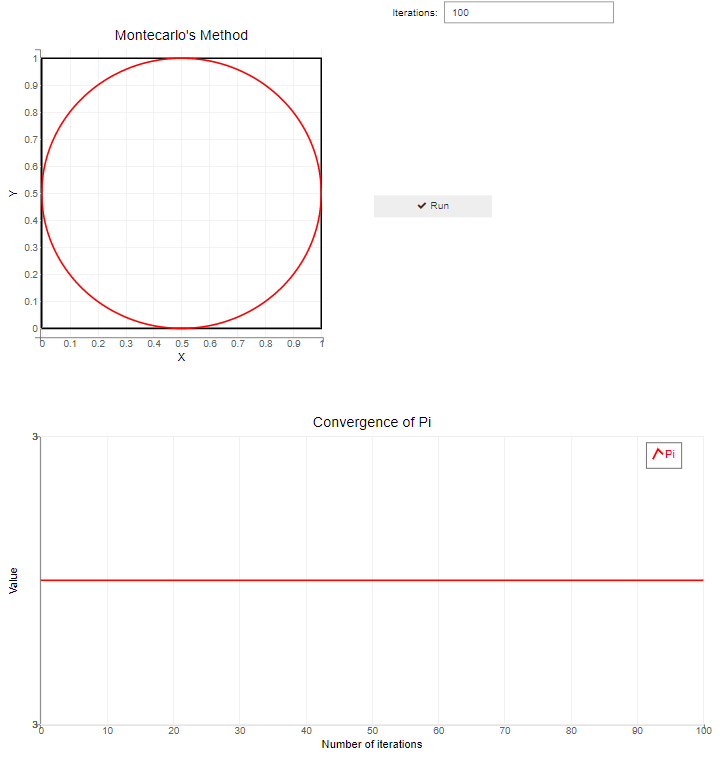
\includegraphics[scale=0.7]{Include/Images/Thesis/Documentation/Visualizers/Randomness/Example 1/Example 1 - 00 - Initial State.png}
    \item Clicked played with 100 default points\\
    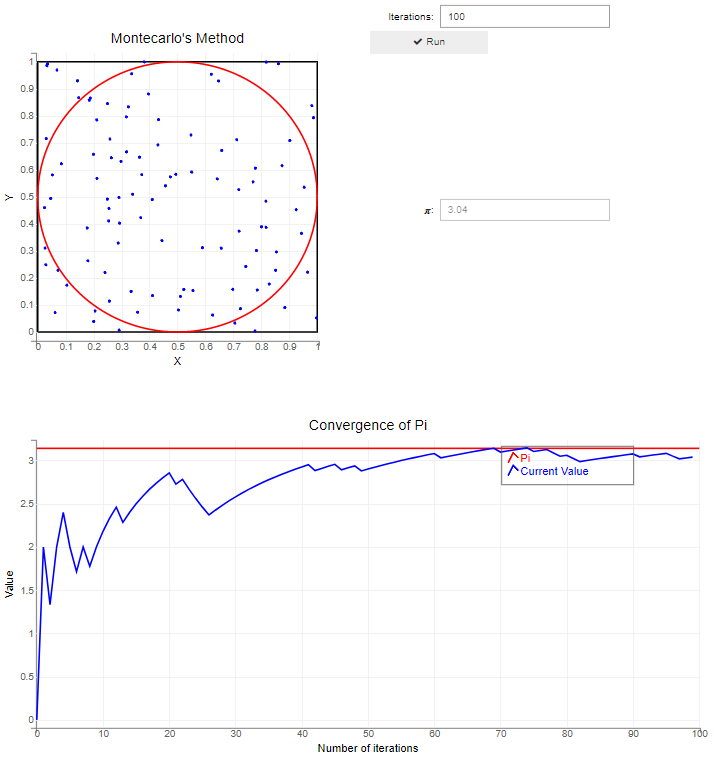
\includegraphics[scale=0.7]{Include/Images/Thesis/Documentation/Visualizers/Randomness/Example 1/Example 1 - 01 - Clicked PLayed.png}
    \item Change number of points to 500 and clicked play\\
    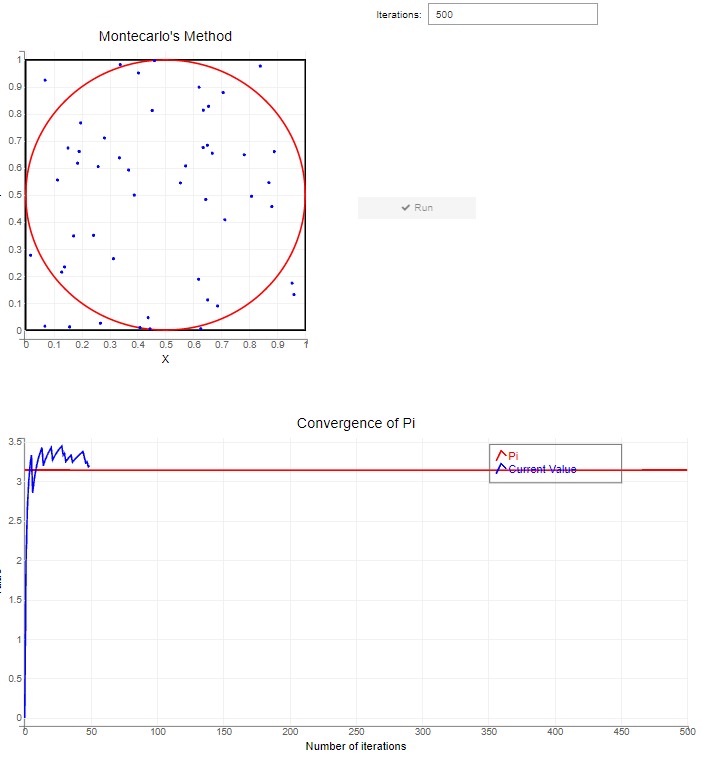
\includegraphics[scale=0.7]{Include/Images/Thesis/Documentation/Visualizers/Randomness/Example 1/Example 1 - 02 - Changed N of points and played.png}
    \item Final of animation playing\\
    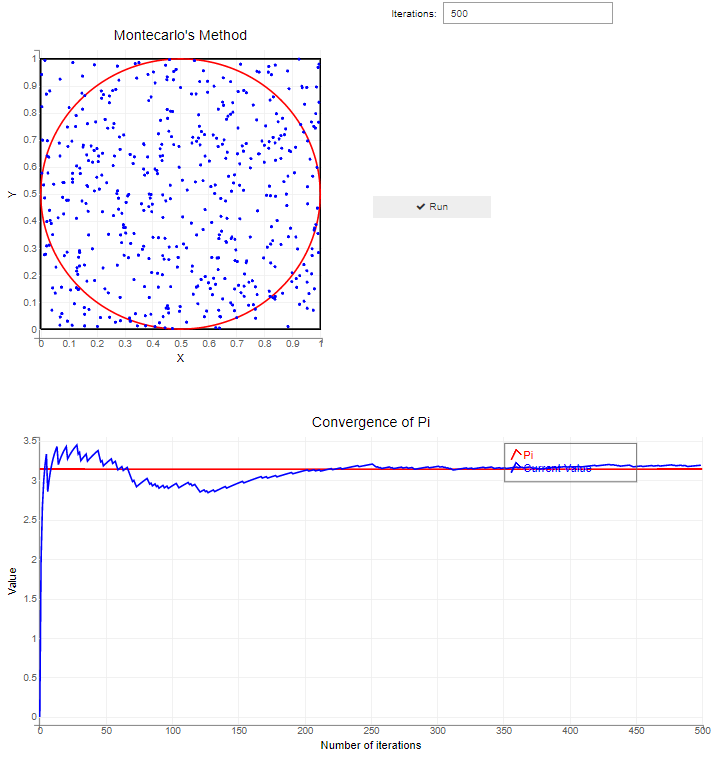
\includegraphics[scale=0.7]{Include/Images/Thesis/Documentation/Visualizers/Randomness/Example 1/Example 1 - 03 - Finished.png}
\end{enumerate}


\paragraph{Example 2: Input arguments and Ill-Generator}
\begin{lstlisting}[language=Python]
from BNumMet.Visualizers.RandomVisualizer import RandomVisualizer
from BNumMet.Random import marsaglia_rand, clear_marsaglia_vars

clear_marsaglia_vars()
randomFunc = lambda: marsaglia_rand(
    base=10, lag_r=2, lag_s=1, carry=0, seed_tuple=(0, 1)
)
randomVisualizer = RandomVisualizer(randomFunc)
randomVisualizer.run()
\end{lstlisting}

\begin{enumerate}
    \item Initial State\\
    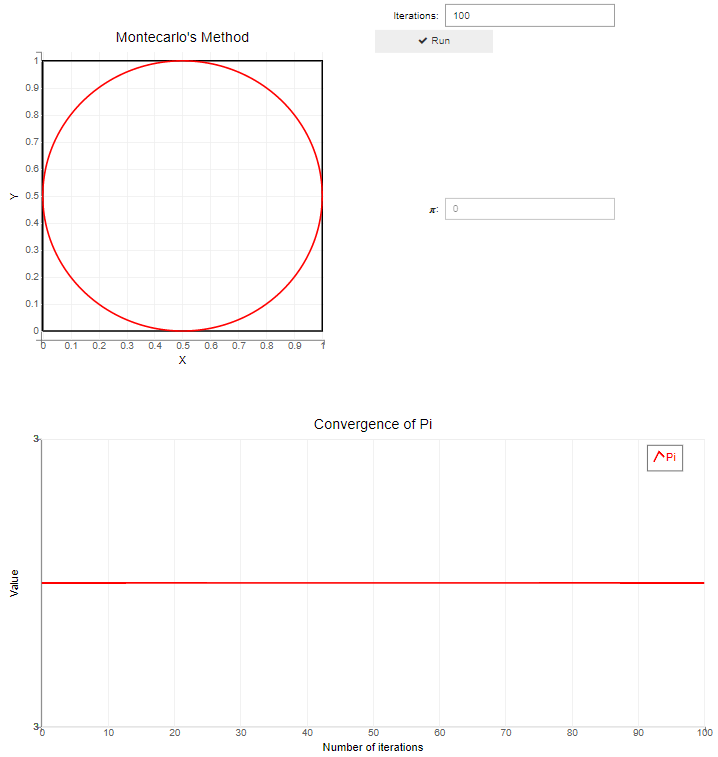
\includegraphics[scale=0.7]{Include/Images/Thesis/Documentation/Visualizers/Randomness/Example 2/Example 2 - 00 - Initial State.png}
    \item Clicked played with 100 default points\\
    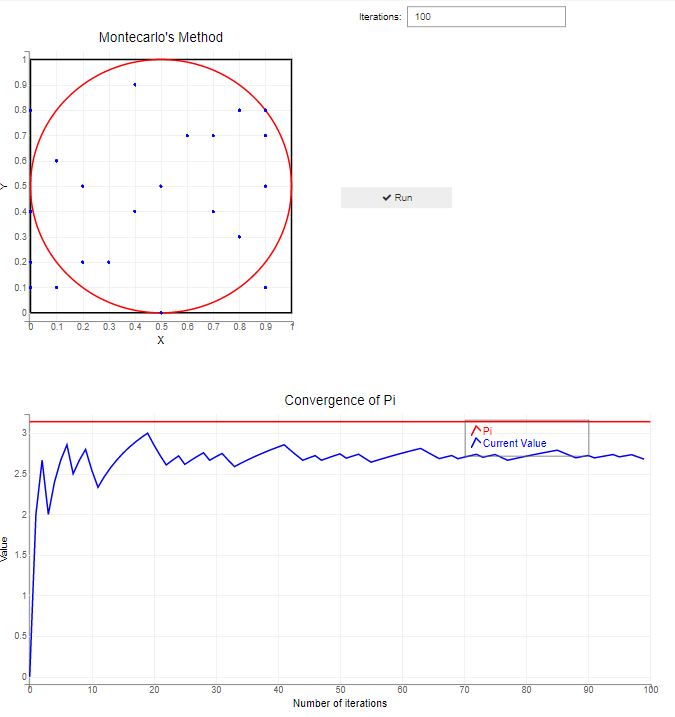
\includegraphics[scale=0.7]{Include/Images/Thesis/Documentation/Visualizers/Randomness/Example 2/Example 2 - 01 - Clicked PLayed.png}
    \item Change number of points to 1000 and clicked play\\
    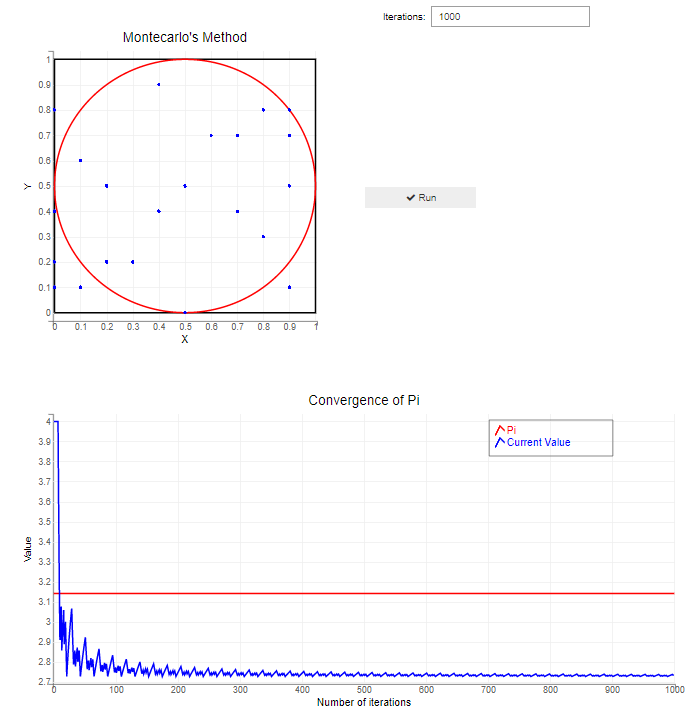
\includegraphics[scale=0.7]{Include/Images/Thesis/Documentation/Visualizers/Randomness/Example 2/Example 2 - 02 - 1000 points played.png}

\end{enumerate}